%//==============================--@--==============================//%
\newpage
\subsection[1.3 Débitos e atraso]{\hspace*{0.075 em}\raisebox{0.2 em}{$\pmb{\drsh}$} Débitos e atraso}
\label{subsec:débitos-e-atraso}

%//==============================--@--==============================//%
\subsubsection[1.3.1 Tipos de Atraso]{$\pmb{\rightarrow}$ Tipos de atraso (\textit{delay})}

\begin{figure}[H]
    \centering
    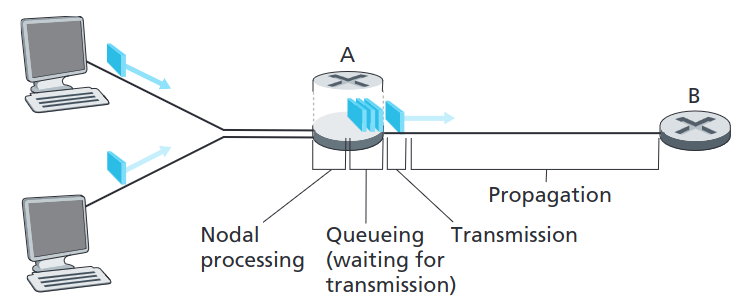
\includegraphics[width = 0.7\linewidth]{img/1/delay.png}
    \caption{Tipos de atraso}
    \label{fig:delay}
\end{figure}

$$
    \boxed{d_{\text{switch}} + d_{\text{queue}} + d_{\text{trans}} + d_{\text{prop}}}
$$


\begin{theo}[\underline{Processing Delay (Atraso de Comutação)}: $\boxed{ d_{\text{switch}} }$]{def:ProcessingDelay}\label{def:ProcessingDelay}
    ``The time required to examine the packet’s header and determine where to direct the packet is part of the \textbf{\textit{processing delay}}. The processing delay can also include other factors, such as the time needed to check for bit-level errors in the packet that occurred in transmitting the packet’s bits from the upstream node to router.''\cite{Kurose2017}
\end{theo}

\begin{theo}[\underline{Queue Delay (Atraso de fila de espera)}: $\boxed{ d_{\text{queue}} }$]{def:QueueDelay}\label{def:QueueDelay}
    ``At the queue, the packet experiences a \textbf{\textit{queuing delay}} as it waits to be transmitted onto the link. The length of the queuing delay of a specific packet will depend on the number of earlier-arriving packets that are queued and waiting for transmission onto the link. ''\cite{Kurose2017}

    \vspace{1 em}
    \noindent \textbf{Nota:} o atraso de fila de espera é dependente da intensidade de tráfego, $La/R$, em que $a$ é dado em $[$packets/s$]$. Se $La/R > 1$ o \textit{rate} de chegada de pacotes excede o \textit{rate} de transmissão, ``the queue will tend to increase without bound and the queuing delay will approach infinity!''\cite{Kurose2017}
\end{theo}

\begin{theo}[\underline{Transmission Delay (Atraso de Transmissão)}: $\boxed{ d_{\text{trans}} }$]{def:TransDelay}\label{def:TransDelay}
    ``The \textbf{\textit{transmission delay}} is $L/R$. This is the amount of time required to push (that is, transmit) all of the packet’s bits into the link. ''\cite{Kurose2017}
\end{theo}

\begin{theo}[\underline{Propagation Delay (Atraso de Propagação)}: $\boxed{ d_{\text{prop}} }$]{def:PropDelay}\label{def:PropDelay}
    ``The \textbf{\textit{propagation delay}} is the distance between two routers divided by the propagation speed. That is, the propagation delay is $d/s$, where $d$ is the distance between router A and router B and $s$ is the propagation speed of the link.''\cite{Kurose2017}
\end{theo}

\renewcommand*{\thefootnote}{\fnsymbol{footnote}}
\footnotetext[4]{%
    \textbf{Nota:} Leia-se $L$ $[$bits$]$ como \textit{length} do pacote, e $R$ $[$bps$]$ como o ritmo de transmissão/capacidade.
}
\renewcommand*{\thefootnote}{\arabic{footnote}}
%//==============================--@--==============================//%
\clearpage
\subsubsection[1.3.2 Exemplos]{$\pmb{\rightarrow}$ Exemplos}
\paragraph[1.3.2.1 Comutação de mensagens vs. comutação de pacotes]{$\pmb{\star}$ Comutação de mensagens \textit{versus} comutação de pacotes}\mbox{}\\[4pt]
{\small
    Considere um comutador com duas linhas de entrada, cada uma com capacidade $10$ Mbit/s, e uma linha de saída com capacidade $20$ Mbit/s. Na primeira linha chegam ao comutador mensagens do tipo A contendo $10$ MB cada e na segunda linha chegam mensagens do tipo B contendo $1$ KB cada.
}

\vspace{1 em}
\begin{figure}[H]
    \centering
    \vspace{-8mm}
    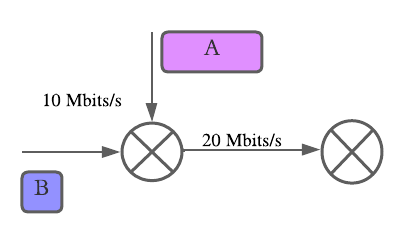
\includegraphics[width=0.4\textwidth]{img/1/diagram.png}
    \hfill\raisebox{4 em}{%
        \parbox{0.55\textwidth}{%
            \noindent \textbf{Comutação de mensagem:} Toda a mensagem é recebida e logo a seguir transmitida se a linha de saída estiver desocupada.
            \vskip 0.5em
            \noindent \textbf{Comutação de pacotes:} A mensagem é seg- mentada em pacotes. Cada pacote é recebido e transmitido por ordem de chegada.
        }
    }
    %\caption{Diagrama de transmissão}
    \label{fig:Dia}
\end{figure}

\vspace{-0.75 em}
\noindent $\blacktriangle$ Assumindo multiplexagem de mensagens, qual é, no pior caso, o atraso a que está sujeita uma mensagem do tipo B, medido desde o momento em que a mensagem chega ao comutador até que o seu último bit é transmitido na linha de saída?

\vspace{0.75 em}
\noindent $\pmb{[\textbf{A}]:}$ O \textbf{pior caso} denota a ocupação da linha de saída pela \underline{mensagem A}. Desta forma, a transmissão de uma mensagem de tipo B terá partida apenas quando toda a mensagem A for transmitida para o terminal de chegada (\textit{store and forward}):

\begin{figure}[H]
    \centering
    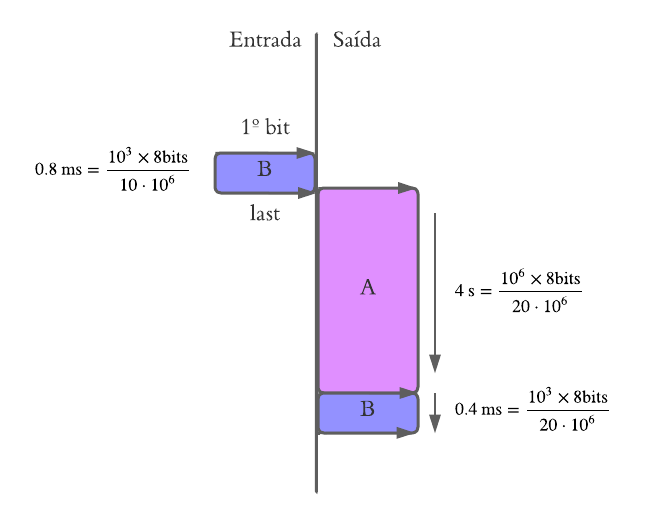
\includegraphics[width = 0.8\linewidth]{img/1/AtrasoB.png}
    %\caption{Diagrama de atraso B}
    \label{fig:AtrasoB}
\end{figure}

\noindent A mensagem B chega imediatamente antes do início da transmissão de A, e aguarda a sua transmissão integral, por fim, ocupa a linha de saída (não é considerado o atraso proveniente da linha de entrada):
$$
    \boxed{\therefore \text{Atraso Total} = 0.4\; \text{ms} + 4\; \text{s} = \pmb{4.0004}\; \textbf{s}}
$$

\clearpage
\noindent $\blacktriangle$ Assumindo multiplexagem de pacotes, cada um com $1$ KB, qual é agora o atraso a que está sujeita uma mensagem do tipo B?

\vspace{-0.5em}
\begin{figure}[H]
    \centering
    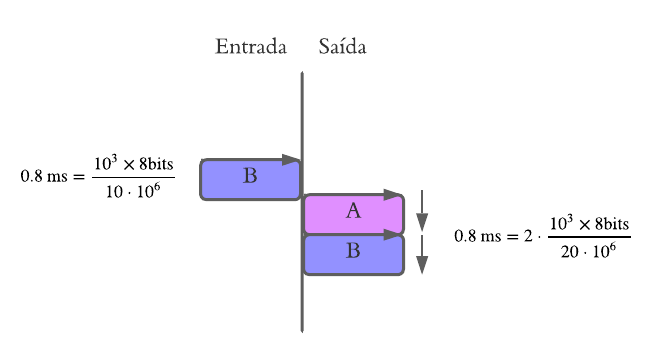
\includegraphics[width = 0.85\linewidth]{img/1/AtrasoBpacket.png}
    %\caption{CAPTION} 
    \label{fig:AtrasoBPacket}
\end{figure}

\noindent $\pmb{[\textbf{A}]:}$ Assumindo multiplexagem por pacotes, o atraso total será dado pelo delay da transmissão dos pacotes $A$ e $B$:
$$
    \boxed{\therefore \text{Atraso Total} = 0.4\; \text{ms} + 0.4\; \text{ms} = \pmb{0.8}\; \textbf{ms}}
$$
\noindent Passa a existir equidade na partilha de recursos de transmissão e comutação (a mensagem B não monopoliza a linha de saída).

\vspace{1.5 em}
\noindent $\blacktriangle$ O que pode dizer relativamente ao atraso sofrido pelas mensagens do tipo A num caso e no outro?

\vspace{0.75 em}
\noindent $\pmb{[\textbf{A1}]:}$ Assumindo multiplexagem por mensagem para transmissão da mensagem A o atraso para o pior caso calculado será idêntico ao já vizualizado na primeira alínea, $4.0004$ s, já que apenas se verifica uma troca na ordem de transmissão. Assim a mensagem A terá de esperar $0.4$ s provenientes da ocupação da linha de transmissão pela mensagem de tipo B e subsequentemente terá de aguardar $4$ s até que todos os seus bits tenham sido transmitidos. 

\vspace{1 em}
\noindent $\pmb{[\textbf{A2}]:}$ Supondo agora comutação de pacotes:

\vspace{-0.5em}
\begin{figure}[H]
    \centering
    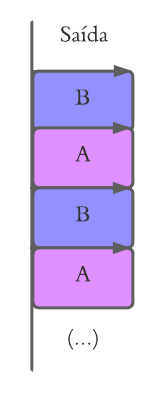
\includegraphics[width = 0.15\linewidth]{img/1/Interleave.png}
    \quad\raisebox{7 em}{%
        \parbox{0.6\textwidth}{%
            \noindent Neste cenário os pacotes de A e de B saem intercalados (\textit{interleaved}). Assim, a mensagem A---composta por $10000$ pacotes---tem um atraso de:
            $$
                \boxed{ d_{\text{total}} = 10000 \cdot \left(2 \cdot \dfrac{10^3 \times 8}{20 \cdot 10^6}\right) = 10^5 \cdot 0.8\, \text{ms} = \pmb{80}\, \textbf{s} }
            $$
            Visto que cada pacote tem um atraso de $0.8$ ms (sempre que um pacote de uma mensagem de tipo A entra no canal, este encontra-se ocupado por uma mensagem de tipo B).
        }
    }
    %\caption{Pacotes Intercalados}
    \label{fig:Interleave}
\end{figure}

%//==============================--@--==============================//%
\clearpage
\paragraph[1.3.2.2 Entrega de um ficheiro ao longo de um caminho]{$\pmb{\star}$ Entrega de um ficheiro ao longo de um caminho}\mbox{}\\[4pt]
{\small
    Considere o envio de um ficheiro contendo 100 KB através de um caminho composto por três troços de fibra óptica interligados por dois comutadores. O primeiro troço tem $100$Km de comprimento e capacidade $10$ Mbit/s; o segundo tem $2.000$ Km de comprimento e capacidade $100$ Mbit/s; e o terceiro tem $4$ Km de comprimento e capacidade 1 Gbit/s. A velocidade de propagação da luz na fibra é de $200.000$ km/s. É usada uma tecnologia de comutação de pacotes.
    
    \vspace{1 em}
    \noindent \textbf{Nota:} Embora seja referida comutação de pacotes, considera-se a dimensão do pacote deprezável face à dimensão do ficheiro
}

\vspace{1 em}
\noindent $\blacktriangle$ Qual o atraso na entrega do ficheiro?

\vspace{-0.75em}
\begin{figure}[H]
    \centering
    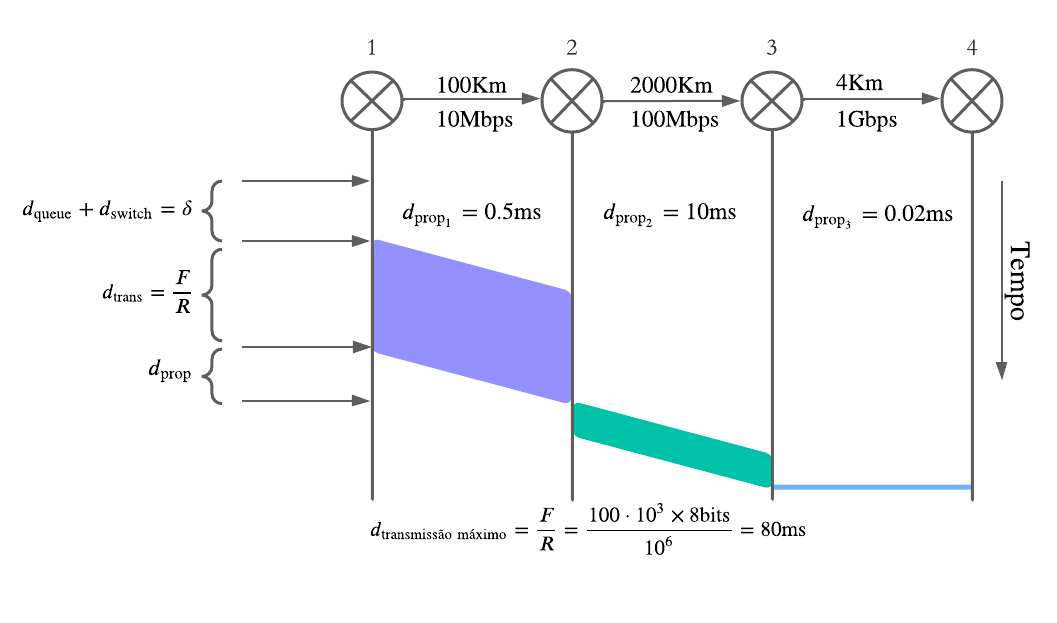
\includegraphics[width = 0.85\linewidth]{img/1/network-delay-diagram.png}
    %\caption{Diagrama de atraso de rede}
    \label{fig:NetworkDelayDiagram}
\end{figure}

\vspace{-1em}
\noindent $\pmb{[\textbf{A}]:}$ Invocando a fórmula do cálculo aproximado da latência na entrega de mensagens com N pacotes ($F = NL$):

\vspace{-1em}
$$
    d_{\text{total}} \approx \delta  + \frac{F}{\displaystyle \min_i\left\{R_i\right\}} + \sum_{i=1}^{n-1} d_{\text{prop},i}
$$

\vspace{-0.25em}
\noindent temos então, para $F = 100$ KB, um atraso: $d_{\text{total}} \approx \delta + 0.5 + 10 + 0.02 + 80 = 90.52\text{ ms} + \delta$.

\vspace{1 em}
\noindent $\blacktriangle$ Quais dos comutadores experimentam uma ocupação da sua fila de espera?

\vspace{0.75 em}
\noindent $\pmb{[\textbf{A}]:}$ Nenhum, os ritmos são crescentes a jusante, i.e, o ritmo de entrada é sempre inferior ao ritmo de saída, o ritmo de crescimento da fila é negativo.

\vspace{1 em}
\noindent $\blacktriangle$ Suponha agora que as capacidades dos dois primeiros troços são trocadas. Isto é: o primeiro troço fica com capacidade $100$ Mbit/s e o segundo fica com capacidade $10$ Mbit/s. Qual o atraso na entrega do ficheiro?

\vspace{0.75 em}
\noindent $\pmb{[\textbf{A}]:}$ O atraso é idêntico ao calculado na primeira alínea. A fórmula é invariante à posição dos comutadores e limitada apenas pela menor capacidade ao longo de toda a transmissão, que continua a ser $10$ Mbits/s.

\vspace{1 em}
\noindent $\blacktriangle$ Qual a ocupação máxima da fila de espera à saída do primeiro comutador? 

\vspace{0.75 em}
\noindent $\pmb{[\textbf{A}]:}$ A fila de espera cresce a um ritmo de $100\text{Mbps} - 10\text{Mbps} = 90\text{Mbps}$, durante $8$ ms (tempo de transmissão assumindo um $R_{\text{entrada}} = 100\text{Mbps}$, como na alinea anterior).
$$
    \text{\underline{Tamanho da fila}} = 90\text{Mbps} \cdot 8\text{ms} = 720000 \text{ bits} = 90 \text{KB} \implies \frac{90\text{KB}}{F} = 0.9 = 90\%
$$
%//==============================--@--==============================//%